% CHAPTER SLIDE
\cscschapter{Introduction}

%%%%
\begin{frame}[fragile]{Introduction to CUDA}
    \begin{info}{The plan}
        \begin{itemize}
            \item learn about the GPU programming model
            \item implement CUDA kernels for simple linear algebra
            \item learn how to orchestrate asynchronous computaion and communication on GPU
            \item a 2D stencil application
        \end{itemize}
    \end{info}

    \begin{info}{Prerequisites}
        \begin{itemize}
            \item I assume C++ knowledge
            \begin{itemize}
                \item I will be using C++11 (the bits that make C++ easier!)
                \item Fortran users consider working with a C++ user
            \end{itemize}
            \item No GPU or graphics experience required
        \end{itemize}
    \end{info}

\end{frame}

%%%%
\begin{frame}[fragile]{What is CUDA?}
    \begin{info}{A superset of C++}
        \begin{itemize}
            \item write CPU code using C++ (C++11 since CUDA 6.5)
            \item write kernels to run on GPU using new keywords
            \item provides special syntax for launching kernels on GPU
        \end{itemize}
    \end{info}

    \begin{info}{GPU specific}
        \begin{itemize}
            \item the CUDA extensions define the \emph{programming model}
            \item PRO : programming model is well suited to GPU
            \item CON : GPU-specific
        \end{itemize}
    \end{info}

    \begin{info}{Extras}
        \begin{itemize}
            \item provides library/API
            \item tools for profiling and debugging
        \end{itemize}
    \end{info}
\end{frame}

%%%%
\begin{frame}[fragile]{Device and Host Memory}
    \begin{center}
        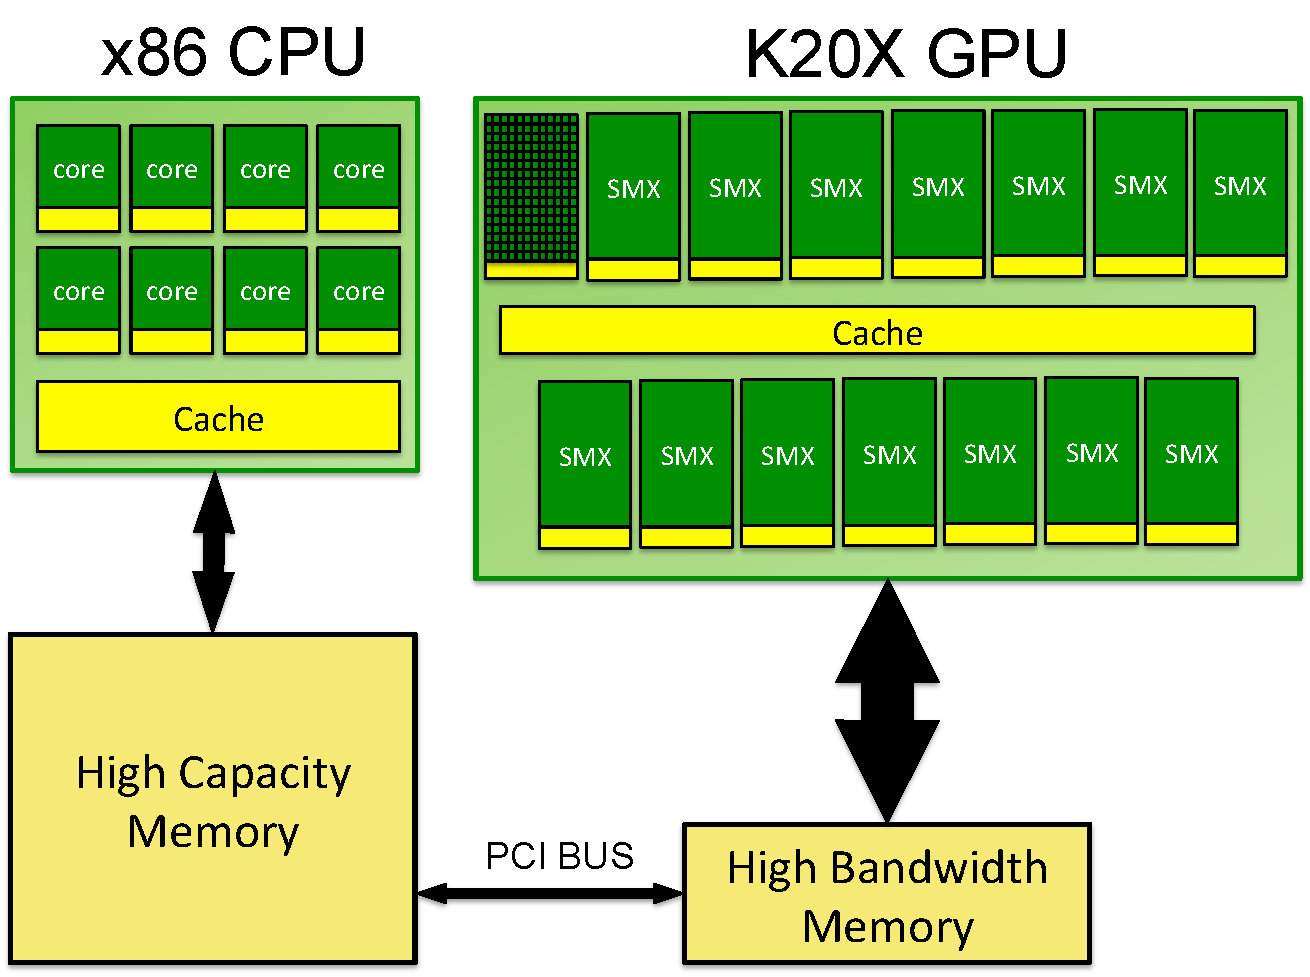
\includegraphics[width=0.9\textwidth]{./images/node.pdf}
    \end{center}
\end{frame}

%%%%%%%%%%%%%%%%%%%%%%%%%%%%%%%%%%%%
\begin{frame}[fragile]{Device and Host Memory}
%%%%%%%%%%%%%%%%%%%%%%%%%%%%%%%%%%%%
    \begin{info}{host and device have separate memory spaces}
        \begin{itemize}
            \item data must be copied between host and device memory via PCI
            \item data must be in device memory for kernels to access
            \item ensure data is in the right memory space \emph{before} computation starts
                \begin{itemize}
                    \item PCIe2 = 6-12 GB/s
                    \item CPU socket = 35-50 GB/s
                    \item K20X  = 180 GB/s
                \end{itemize}
        \end{itemize}
    \end{info}

\end{frame}

% CHAPTER SLIDE
\cscschapter{Keeping it local}

%%%%%%%%%%%%%%%%%%%%%%%%%%%%%%%%%%%%%%%%%%%%
\begin{frame}[fragile]{coordination on SMX}
%%%%%%%%%%%%%%%%%%%%%%%%%%%%%%%%%%%%%%%%%%%%
    \begin{info}{}
        Section about using shared resources on an SMX in a thread block
        \begin{itemize}
            \item shared memory
            \item \lst{__synch_threads()}
        \end{itemize}
        Two examples that stick to one thread block
        \begin{itemize}
            \item reverse string
            \item dot product
        \end{itemize}
    \end{info}

\end{frame}

